\section{Results}
\label{sec:results}

\subsection{Performance}

\begin{itemize}
	\item How long does it take to do matrix calculation for one consensus?
\end{itemize}

\subsection{Churn rate analysis}
Narrow distribution, with 99.9\% of all churn values being in the interval $[0, 0.07624282]$.

\begin{table}[ht]
	\centering
	\begin{tabular}{llllll}
	Min. & 1st Qu. & Median & Mean & 3rd Qu. & Max. \\
	\hline
	0.00423 & 0.01782 & 0.02647 & 0.02930 & 0.03972 & 0.54500 \\
	\end{tabular}
	\caption{Summary of churn rate distribution.}
	\label{tab:churn_distribution}
\end{table}

\begin{figure}[t]
	\centering
	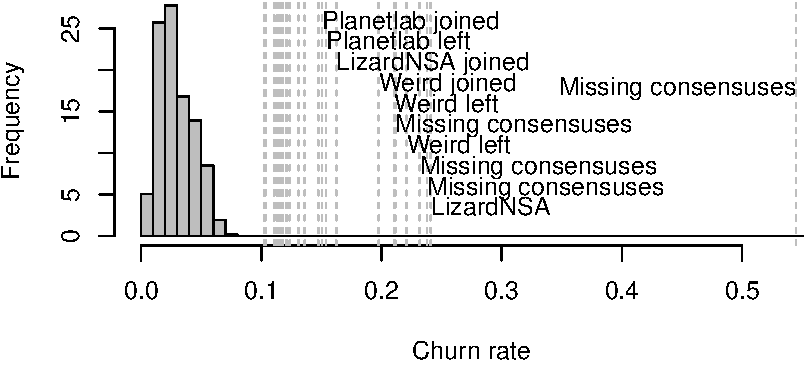
\includegraphics[width=0.49\textwidth]{diagrams/churn.pdf}
	\caption{Histogram of the churn rates between all 67,671 consensuses.  21
		outliers in the interval $[0.1, 0.15[$ are marked, and 11 outliers in
		the interval $[0.15, 0.54499]$ are also labelled.}
	\label{fig:churn}
\end{figure}

\subsection{Fingerprint anomalies}

\begin{figure}[t]
	\centering
	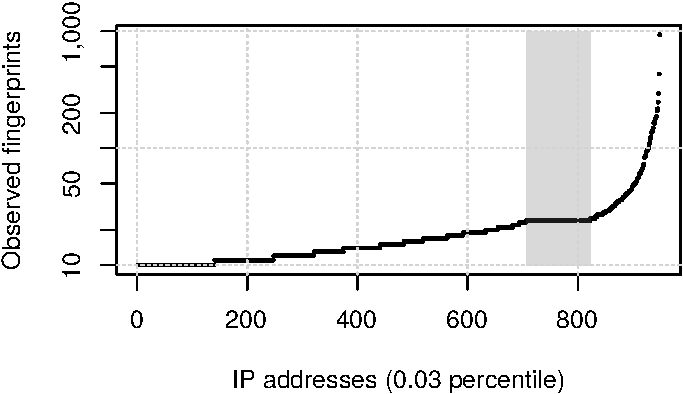
\includegraphics[width=0.49\textwidth]{diagrams/fingerprints.pdf}
	\caption{Foo.}
	\label{fig:fingerprints}
\end{figure}

\begin{figure*}[t]
	\centering
	
\includegraphics[width=\textwidth]{diagrams/uptimes.pdf}
	\caption{A visualization of the uptime pattern of Tor relays.  The matrix'
	x-axis represents a Tor relay, one per column.  The y-axis represents a
	relay's uptime status in one consensus file.  A black pixel indicates that
	the relay was online, and a white pixel indicates that it was offline.  Red
	pixels marks similar relays, as determined by Algorithm~\ref{alg:uptime}.}
	\label{fig:fingerprints}
\end{figure*}

There is an interesting plateau at 24, encompassing xx relays.

\subsection{Sybil groups}
\label{sec:sybil_groups}
Table~\ref{tab:sybils} contains all the Sybil groups we identified.  For every
group, we document when it first appeared in the Tor network, its ``name,''
size, and a description of its characteristics.

The number of relays refers to the maximum amount of Sybils that was online at
any point in time.

\begin{table*}[t]
\centering
\begin{tabular}{l c c p{10cm}}
\textbf{First seen} & \textbf{Group ID} & \textbf{\# of relays} & \textbf{Characteristics} \\
\hline
2015-07-10 & DenkoNet & 58 & Hosted on Amazon AWS.  Only online for one consensus. \\
2015-07-02 & cloudvps & 55 & Unknown. \\
2015-06-29 & onion rewrite & 55 & Transparent onion URL rewriting. \\
2015-06-17 & 1jabberat & X & not good. \\
2015-06-05 & hsdirscanner2 & 105 & Scanning HSDirs. \\
2015-06-03 & abcd & 28 & Changing fingerprints. \\
2015-05-29 & facebook hsdirs & 6 & Became HSDirs responsible for facebook.  \\
2015-05-20 & hsdirscanner1 & 102 & Scanning HSDirs. \\
2015-04-22 & sigaint & 83 & Targeting (at least) sigaint.org. \\
2015-03-11 & bitcoin-redirect & 24 & Attacking Bitcoin sites by redirecting to own web server. \\
2015-XX-YY & default & many & Likely a Windows-powered botnet.  The group
features wide, geographical distribution, which is uncommon for typical Tor
relays. \\
2013-02-03 & AmazonEC2 & XX & Changed their fingerprint exactly 24 times. \\
% Shared: nickname, IP address, port, platform, version.
2014-12-26 & LizardNSA & 3,347 & \\
2014-12-26 & FuslVZTOR & 246 & \\
2014-12-30 & Anonpoke & 284 & \\
\end{tabular}
\caption{Sybil groups identified by our system.  Our raw data is available
online at {\normalfont\url{https://nymity.ch/sybilhunting/}}.}
\label{tab:sybils}
\end{table*}

\paragraph{default}
Likely a Windows-powered botnet.

\paragraph{LizardNSA}
All relays were hosted in the Google Cloud, and only online for nine hours,
until the directory authorities started rejecting them.  The majority of
machines were middle relays (96\%), but the attackers also started some exit
relays (4\%).  The Sybils were set up to be hidden service directories, but the
relays were taken offline before they were assigned the \texttt{HSDir} flag.  If
all relays would have obtained the \texttt{HSDir} flag in time, they would have
constituted almost 50\% of all hidden service directories; the median number of
hidden service directories on Dec. 26 was 3,551.

\paragraph{FuslVZTOR}
All machines were middle relays and hosted in 212.38.181.0/24, a VPS provider's
network in the UK.  The directory authorities started rejecting the relays five
hours after they were first seen.  The relays advertized the default bandwidth
of 1 GiB/s and used seemingly randomly determined ports.  Other than happening
in parallel to the LizardNSA attack, there is no reason to believe that both
incidents are related.

\paragraph{Anonpoke}
The relays were online for four hours until they were rejected.  All relays were
hosted by a VPS provider in the US, with the curious exception of a single relay
that was hosted in the UK, and running a different Tor version.  The relays
advertized the default bandwidth of 1 GiB/s on port 9001 and 9030.  All relays
were middle relays and running as directory mirror.

\subsection{Other anomalies}
\begin{itemize}
	\item Some events with unexpectedly high network churn.  Generally, churn
		is not problematic.  It can be problematic, however, for guard relays,
		if they change their IP addresses.

	\item Several relays changed their fingerprint an unusually high amount of
		times.  Cause often misconfiguration, but in some cases likely attacks
		on Tor's DHT.
\end{itemize}
